% ============================================================
%  PRÉSENTATION BEAMER — Projet PF22 — Seconde Présentation
%  Auteur : Ivann Vasic — UTBM — Mars–Juin 2026
% ============================================================
\documentclass[aspectratio=169, 10pt]{beamer}

% ============================================================
%  PAQUETS
% ============================================================
\usepackage[utf8]{inputenc}
\usepackage[T1]{fontenc}
\usepackage[french]{babel}
\usepackage{lmodern}
\usepackage{helvet}
\renewcommand{\familydefault}{\sfdefault}
\usepackage{microtype}
\usepackage{graphicx}
\usepackage{booktabs}
\usepackage{tabularx}
\usepackage{multirow}
\usepackage{array}
\usepackage{colortbl}
\usepackage{tikz}
\usetikzlibrary{shapes.geometric, arrows.meta, positioning, fit, backgrounds, calc, shadows.blur}
\usepackage{xcolor}
\usepackage{pgfplots}
\pgfplotsset{compat=1.18}
\usepackage{amsmath}
\usepackage{amssymb}
\usepackage{fontawesome5}

% ============================================================
%  PALETTE
% ============================================================
\definecolor{primary}{RGB}{18,36,66}
\definecolor{primarydk}{RGB}{10,22,44}
\definecolor{accent}{RGB}{14,165,164}
\definecolor{accentlight}{RGB}{186,230,228}
\definecolor{gold}{RGB}{217,164,65}
\definecolor{goldlight}{RGB}{246,228,192}
\definecolor{paper}{RGB}{248,249,251}
\definecolor{card}{RGB}{255,255,255}
\definecolor{rule}{RGB}{222,227,235}
\definecolor{ink}{RGB}{28,36,52}
\definecolor{muted}{RGB}{110,122,142}
\definecolor{hfcolor}{RGB}{31,81,140}
\definecolor{bfcolor}{RGB}{142,152,170}
\definecolor{success}{RGB}{46,139,87}
\definecolor{warn}{RGB}{205,133,63}
\definecolor{danger}{RGB}{176,58,58}

% ============================================================
%  THÈME BEAMER
% ============================================================
\usetheme{default}
\usecolortheme{default}
\setbeamertemplate{navigation symbols}{}
\setbeamertemplate{frametitle continuation}{}

\setbeamercolor{background canvas}{bg=paper}
\setbeamercolor{normal text}{fg=ink}
\setbeamercolor{frametitle}{fg=primary, bg=paper}
\setbeamerfont{frametitle}{series=\bfseries, size=\large}
\setbeamercolor{title}{fg=white}
\setbeamercolor{subtitle}{fg=accentlight}
\setbeamercolor{author}{fg=accentlight}
\setbeamercolor{date}{fg=muted}
\setbeamercolor{item}{fg=accent}
\setbeamercolor{subitem}{fg=muted}
\setbeamertemplate{itemize item}{\color{accent}\small\faAngleRight}
\setbeamertemplate{itemize subitem}{\color{muted}\scriptsize$\blacktriangleright$}
\setbeamerfont{block title}{series=\bfseries, size=\small}

\setbeamertemplate{footline}{%
  \begin{beamercolorbox}[wd=\paperwidth, ht=0.5cm, dp=0.25cm]{footline}%
    \begin{tikzpicture}[overlay, remember picture]
      \draw[rule, line width=0.4pt]
        ([xshift=0.7cm, yshift=0.72cm]current page.south west) --
        ([xshift=-0.7cm, yshift=0.72cm]current page.south east);
      \node[anchor=west, text=muted, font=\scriptsize]
        at ([xshift=0.7cm, yshift=0.38cm]current page.south west)
        {Ivann Vasic\,\textbf{\textbar}\,Projet PF22\,\textbf{\textbar}\,UTBM 2026};
      \node[anchor=east, text=muted, font=\scriptsize]
        at ([xshift=-2.4cm, yshift=0.38cm]current page.south east)
        {Approche Multi-Fidélité - Validations};
      \node[anchor=east, text=primary, font=\scriptsize\bfseries]
        at ([xshift=-0.7cm, yshift=0.38cm]current page.south east)
        {\insertframenumber\,/\,\inserttotalframenumber};
    \end{tikzpicture}%
  \end{beamercolorbox}%
}

\setbeamertemplate{frametitle}{%
  \nointerlineskip%
  \vspace{0.25cm}%
  \begin{beamercolorbox}[wd=\paperwidth, ht=0.85cm, dp=0.1cm, leftskip=0.8cm, rightskip=0.8cm]{frametitle}%
    \begin{tikzpicture}[overlay]
      \fill[accent] (-0.45cm, -0.05cm) rectangle (-0.15cm, 0.62cm);
    \end{tikzpicture}%
    {\usebeamerfont{frametitle}\color{primary}\insertframetitle}%
    \ifx\insertframesubtitle\empty\else
      \hfill{\color{muted}\footnotesize\textit{\insertframesubtitle}}%
    \fi\\[-0.1em]
    \textcolor{rule}{\rule{\dimexpr\paperwidth-1.6cm\relax}{0.4pt}}%
  \end{beamercolorbox}%
  \vspace{0.1cm}%
}

\setbeamercolor{block title}{bg=primary, fg=white}
\setbeamercolor{block body}{bg=card, fg=ink}
\setbeamercolor{block title alerted}{bg=danger, fg=white}
\setbeamercolor{block body alerted}{bg=danger!6, fg=ink}
\setbeamercolor{block title example}{bg=success, fg=white}
\setbeamercolor{block body example}{bg=success!7, fg=ink}

\title{\textbf{Validation et Nouvelles Analyses}}
\subtitle{par Approche Multi-Fidélité — 2nde Présentation Intermédiaire}
\author{Ivann Vasic}
\institute{UTBM --- Université de Technologie de Belfort-Montbéliard}
\date{Avancement des travaux --- Juin 2026}

\newcolumntype{L}[1]{>{\raggedright\arraybackslash}p{#1}}
\newcolumntype{C}[1]{>{\centering\arraybackslash}p{#1}}
\newcommand{\card}[2][card]{%
  \tikz[baseline=(x.base)]{\node[fill=#1, rounded corners=2pt, inner sep=4pt,
    drop shadow={shadow xshift=0pt, shadow yshift=-0.4pt, opacity=0.08}] (x) {#2};}%
}
% Valeur ± écart-type (multi-seed) compacte
\newcommand{\pms}[2]{#1{\tiny\,$\pm$#2}\,\%}

% ============================================================
\begin{document}
% ============================================================

% ============================================================
%  SLIDE DE TITRE
% ============================================================
{
\setbeamertemplate{footline}{}
\setbeamertemplate{frametitle}{}
\begin{frame}[plain]
  \begin{tikzpicture}[overlay, remember picture]
    \fill[primarydk] (current page.south west) rectangle (current page.north east);
    \shade[top color=primary, bottom color=primarydk]
      (current page.south west) rectangle (current page.north east);
    \fill[accent, opacity=0.10] ([xshift=-3cm, yshift=-1cm]current page.north east) circle (5.5cm);
    \fill[accent, opacity=0.15] ([xshift=-1.5cm, yshift=-2cm]current page.north east) circle (3cm);
    \fill[gold, opacity=0.18] ([xshift=-0.5cm, yshift=-1cm]current page.north east) circle (1.2cm);
    \fill[accent] (current page.south west) rectangle ([xshift=0.18cm]current page.north west);

    \node[anchor=north west, text=accentlight, font=\footnotesize\bfseries, text width=10cm]
      at ([xshift=0.95cm, yshift=-0.7cm]current page.north west)
      {UNIVERSITÉ DE TECHNOLOGIE DE BELFORT-MONTBÉLIARD};
    \node[anchor=north west, text=muted, font=\scriptsize]
      at ([xshift=0.95cm, yshift=-1.15cm]current page.north west)
      {PROJET PF22\quad\textbullet\quad DÉPARTEMENT INFORMATIQUE};

    \draw[accent, line width=0.8pt]
      ([xshift=0.95cm, yshift=-1.55cm]current page.north west) --
      ([xshift=2.5cm, yshift=-1.55cm]current page.north west);

    \node[anchor=north west, text=white, font=\fontsize{24}{28}\bfseries\selectfont, text width=12cm]
      at ([xshift=0.95cm, yshift=-2cm]current page.north west)
      {Avancements \& Validation};
    \node[anchor=north west, text=white, font=\fontsize{24}{28}\bfseries\selectfont, text width=12cm]
      at ([xshift=0.95cm, yshift=-2.95cm]current page.north west)
      {Approche Multi-Fidélité};
    \node[anchor=north west, text=accent, font=\Large\bfseries, text width=12cm]
      at ([xshift=0.95cm, yshift=-3.95cm]current page.north west)
      {2\textsuperscript{nde} Présentation Intermédiaire};

    \node[anchor=north west, text=accentlight!85, font=\small, text width=11cm]
      at ([xshift=0.95cm, yshift=-4.85cm]current page.north west)
      {Validation multi-seed, second dataset (Imagewoof) et nouvelles analyses : robustesse, frontière de Pareto coût/précision, sensibilité au ratio de coût.};

    \draw[accent, line width=0.6pt]
      ([xshift=0.95cm,  yshift=1.85cm]current page.south west) --
      ([xshift=6cm, yshift=1.85cm]current page.south west);

    \node[anchor=west, text=white, font=\normalsize\bfseries]
      at ([xshift=0.95cm, yshift=1.4cm]current page.south west)
      {Ivann Vasic};
    \node[anchor=west, text=accentlight, font=\footnotesize]
      at ([xshift=0.95cm, yshift=0.95cm]current page.south west)
      {UTBM};
    \node[anchor=west, text=muted, font=\scriptsize]
      at ([xshift=0.95cm, yshift=0.45cm]current page.south west)
      {Mars -- Juin 2026};
  \end{tikzpicture}
\end{frame}
}

% ============================================================
%  SECTION 1 : RAPPEL & PLAN
% ============================================================
\begin{frame}{Rappel Express du Contexte}
\framesubtitle{L'apprentissage Multi-Fidélité en une diapositive}
  \begin{columns}[T]
    \begin{column}{0.65\textwidth}
      \textbf{\color{primary}Principe Fondamental :}
      Remplacer à budget réduit la majorité des données coûteuses (\textit{Haute Fidélité, HF}) par des données dégradées (\textit{Basse Fidélité, BF}) sans perte de performance.
      
      \medskip
      \textbf{\color{primary}Cadre Expérimental :}
      \begin{itemize}\setlength\itemsep{4pt}
        \item \textbf{Modèle} : ResNet-18 sans poids pré-entraînés.
        \item \textbf{Dégradation} : Downsampling $224 \rightarrow 64 \rightarrow 224$ + Bruit Gaussien + Compression JPEG.
        \item \textbf{Coûts} : Mesurés en Crédits d'Annotation (\textbf{CA}). $1$ HF = $10$ CA ; $1$ BF $\approx$ $1$ CA.
        \item \textbf{Mélange type} : 10\% HF + 90\% BF.
      \end{itemize}
    \end{column}
    \begin{column}{0.32\textwidth}
      \centering
      \begin{tikzpicture}[font=\small]
        \node[rounded corners=4pt, fill=card, draw=hfcolor, line width=1pt,
              text width=3.5cm, align=center, minimum height=1cm,
              drop shadow={shadow xshift=0pt, shadow yshift=-1pt, opacity=0.1}] (hf) at (0, 1.8)
          {{\color{hfcolor}\faCamera}\quad\textbf{\color{hfcolor}Données HF}\\[1pt] \footnotesize Nettes (10 CA) / 10\%};

        \node[rounded corners=4pt, fill=card, draw=bfcolor, line width=1pt,
              text width=3.5cm, align=center, minimum height=1cm,
              drop shadow={shadow xshift=0pt, shadow yshift=-1pt, opacity=0.1}] (bf) at (0, 0)
          {{\color{bfcolor}\faLowVision}\quad\textbf{\color{bfcolor}Données BF}\\[1pt] \footnotesize Dégradées (1 CA) / 90\%};

        \draw[Stealth-Stealth, thick, accent, dashed] (hf) -- (bf);
      \end{tikzpicture}
    \end{column}
  \end{columns}
\end{frame}

% ============================================================
%  SECTION 2 : NOUVEL ENVIRONNEMENT (WANDB / GUACAMOLE)
% ============================================================
\begin{frame}{Nouveautés : Modernisation de l'Environnement}
\framesubtitle{WandB, Guacamole}
  \begin{columns}[T]
    \begin{column}{0.48\textwidth}
      \textbf{\color{hfcolor}\faDesktop\ Apache Guacamole}
      \begin{itemize}\footnotesize\setlength\itemsep{2pt}
        \item \textbf{Avant} : Dépendance à Google Colab (limites de sessions, déconnexions).
        \item \textbf{Aujourd'hui} : Accès direct et dédié à un frontal GPU via connexion distante.
        \item \textbf{Gain} : Exécutions nettement plus rapides et continues pour la validation lourde (Multi-seeds).
      \end{itemize}
    \end{column}
    \begin{column}{0.48\textwidth}
      \textbf{\color{accent}\faChartLine\ Weights \& Biases (\textit{WandB})}
      \begin{itemize}\footnotesize\setlength\itemsep{2pt}
        \item Implémentation du système de \textit{tracking}.
        \item Comparaison en direct des métriques de \textbf{3 seeds d'exécution} (Moyenne $\pm$ Écart-type).
        \item Suivi des ressources de la carte graphique.
      \end{itemize}
    \end{column}
  \end{columns}
\end{frame}

% ============================================================
%  SECTION 3 : VALIDATION CROISEE IMAGEWOOF
% ============================================================
\begin{frame}{Un Nouveau Dataset : Validation Croisée sur Imagewoof}
  Afin de garantir que les bénéfices des stratégies multi-fidélité ne sont pas propres au dataset \textbf{Animals-10}, un second jeu de données a été ajouté à la méthodologie.

  \vspace{0.6cm}
  \begin{columns}[T]
    \begin{column}{0.48\textwidth}
      \begin{exampleblock}{Animals-10 (Le terrain d'expérimentation)}
        \begin{itemize}\footnotesize
          \item 26 179 images, 10 classes distinctes (chat, éléphant, papillon...).
          \item Classification "générique".
          \item Volume suffisant pour un entraînement robuste \textit{from scratch}.
        \end{itemize}
      \end{exampleblock}
    \end{column}
    \begin{column}{0.48\textwidth}
      \begin{alertblock}{Imagewoof (Le Crash-Test)}
        \begin{itemize}\footnotesize
          \item 12 954 images, 10 races de chiens !
          \item Classification \textit{fine-grained} : visuellement très difficiles à séparer face au flou.
          \item Volume divisé par 2 $\rightarrow$ met sous pression la stabilité des stratégies.
        \end{itemize}
      \end{alertblock}
    \end{column}
  \end{columns}
  
  \vspace{0.3cm}
  \begin{center}
    \footnotesize\textbf{\color{primary}Objectif :} Une stratégie validée conjointement sur Animals-10 et Imagewoof est jugée robuste. Les \textbf{3 seeds} garantissent des intervalles de confiance rigoureux.
  \end{center}
\end{frame}

\begin{frame}{Redéfinition et affinement des Métriques}
  \begin{columns}[T]
    \begin{column}{0.45\textwidth}
      \textbf{\color{primary}Trois Coûts Analysés}
      \begin{itemize}\footnotesize\setlength\itemsep{4pt}
        \item \textbf{Coût Donnée (CA)} : Acquisition brute. (10 CA par image HF, $\approx$1 CA par BF). Payé 1 seule fois.
        \item \textbf{Coût Calcul} : Volume brut de calcul (N images traitées $\times$ Epochs).
        \item \textbf{Coût Total} : Le cumulatif pondéré. Reflète la vraie charge (N images traitées $\times$ prix unitaire $\times$ Epochs). C'est là que l'approche justifie son efficience !
      \end{itemize}
    \end{column}
    
    \begin{column}{0.50\textwidth}
      \textbf{\color{primary}Intégration d'incertitudes Statistiques}
      Toutes les expériences présentées désormais sont \textbf{la moyenne de 3 Seeds aléatoires} avec leur Écart-type.
      
      \vspace{0.3cm}
    \end{column}
  \end{columns}
\end{frame}

% ============================================================
%  SECTION 4 : BASELINES (COTE A COTE)
% ============================================================
\begin{frame}{Rappel : Baselines (Borne Min \& Borne Max)}
\framesubtitle{Animals-10 vs Imagewoof}
  
  \begin{columns}[T]
    \begin{column}{0.48\textwidth}
      \centering
      \textbf{ANIMALS-10} (Jeu normal)\\
      \vspace{0.2cm}
      \scriptsize
      \renewcommand{\arraystretch}{1.3}
      \begin{tabular}{@{}lC{2cm}C{1.2cm}@{}}
        \toprule
        \color{primary}\textbf{Modèle} & \color{primary}\textbf{Test HF} & \color{primary}\textbf{Coût (CA)} \\
        \midrule
        \rowcolor{hfcolor!8}BL 1 (HF seu.) & \pms{54,3}{2,2} & 470k \\
        \rowcolor{bfcolor!10}BL 2 (BF seu.) & \pms{61,3}{6,3} & \textbf{424k} \\
        \rowcolor{accent!12}BL 3 (Mixte)   & \textbf{\pms{74,0}{3,0}} & 894k \\
        \bottomrule
      \end{tabular}
    \end{column}
    \begin{column}{0.48\textwidth}
      \centering
      \textbf{IMAGEWOOF} (\textit{Fine-grained})\\
      \vspace{0.2cm}
      \scriptsize
      \renewcommand{\arraystretch}{1.3}
      \begin{tabular}{@{}lC{2cm}C{1.2cm}@{}}
        \toprule
        \color{primary}\textbf{Modèle} & \color{primary}\textbf{Test HF} & \color{primary}\textbf{Coût} \\
        \midrule
        \rowcolor{hfcolor!8}BL 1 (HF seu.) & \pms{25,0}{4,1} & 179k \\
        \rowcolor{bfcolor!10}BL 2 (BF seu.) & \pms{42,7}{2,8} & 162k \\
        \rowcolor{accent!12}BL 3 (Mixte)   & \textbf{\pms{50,3}{2,5}} & 342k \\
        \bottomrule
      \end{tabular}
    \end{column}
  \end{columns}

  \vspace{0.5cm}
  \begin{block}{\footnotesize Constat Validé sur les 2 datasets}
    \footnotesize La hiérarchie \textbf{BL3 $>$ BL2 $>$ BL1} est strictement répétée. \\
    L'effondrement de la classification fine-grained (Imagewoof) est fort, mais \textbf{le "Paradoxe de la Quantité"} (BL2 qui bat BL1 malgré son flou, simplement car + de volume) réagit de manière identique !
  \end{block}
\end{frame}

% ============================================================
%  SECTION 5 : STRATEGIE 1
% ============================================================
\begin{frame}{Validation Stratégie 1 : \textit{Transfer Learning Séquentiel}}

  \begin{columns}[T]
    \begin{column}{0.48\textwidth}
      \centering
      \textbf{ANIMALS-10}\\
      \vspace{0.2cm}
      \scriptsize
      \renewcommand{\arraystretch}{1.3}
      \begin{tabular}{@{}lL{1.9cm}C{1.3cm}@{}}
        \toprule
        \color{primary}\textbf{Modèle} & \color{primary}\textbf{HF} & \color{primary}\textbf{Coût} \\
        \midrule
        \rowcolor{accent!10}BL 3 (Mixte)        & \pms{74,0}{3,0} & 894k CA \\
        \rowcolor{success!20}\textbf{Stratégie 1} & \textbf{\pms{78,4}{0,7}} & \textbf{400k CA} \\
        \bottomrule
      \end{tabular}
    \end{column}
    \begin{column}{0.48\textwidth}
      \centering
      \textbf{IMAGEWOOF}\\
      \vspace{0.2cm}
      \scriptsize
      \renewcommand{\arraystretch}{1.3}
      \begin{tabular}{@{}lL{1.9cm}C{1.3cm}@{}}
        \toprule
        \color{primary}\textbf{Modèle} & \color{primary}\textbf{HF} & \color{primary}\textbf{Coût} \\
        \midrule
        \rowcolor{accent!10}BL 3 (Mixte)        & \pms{50,3}{2,5} & 342k CA \\
        \rowcolor{success!20}\textbf{Stratégie 1} & \textbf{\pms{52,0}{0,7}} & \textbf{153k CA} \\
        \bottomrule
      \end{tabular}
    \end{column}
  \end{columns}

  \vspace{0.5cm}
  \begin{columns}[T]
    \begin{column}{0.1\textwidth}
      \centering
      {\Huge\color{success}\faTrophy}
    \end{column}
    \begin{column}{0.85\textwidth}
      \textbf{\color{primary}Vainqueur Incontesté}
      \begin{itemize}\footnotesize
        \item \textbf{Meilleur Test HF} sur les \textbf{deux} datasets : bat la borne supérieure BL3 (+4,4 pts Animals, +1,7 pt Imagewoof).
        \item \textbf{Le plus stable} : écart-type le plus faible ($\pm0,7$) sur 3 seeds.
        \item À \textbf{coût données identique}, \textbf{coût total / calcul $\approx$ divisé par 2} vs BL3.
      \end{itemize}
    \end{column}
  \end{columns}

\end{frame}

% ============================================================
%  SECTION 6 : STRATEGIE 2
% ============================================================
\begin{frame}{Validation Stratégie 2 : \textit{Co-training avec Pondération}}

  \begin{columns}[T]
    \begin{column}{0.48\textwidth}
      \centering
      \textbf{ANIMALS-10}\\
      \vspace{0.2cm}
      \scriptsize
      \renewcommand{\arraystretch}{1.3}
      \begin{tabular}{@{}lL{1.9cm}C{1.2cm}@{}}
        \toprule
        \color{primary}\textbf{Modèle} & \color{primary}\textbf{HF} & \color{primary}\textbf{Coût} \\
        \midrule
        \rowcolor{bfcolor!10}BL 2 (BF)  & \pms{61,3}{6,3} & 424k \\
        \rowcolor{accent!10}BL 3 (Mixte)        & \pms{74,0}{3,0} & 894k \\
        \rowcolor{warn!20}\textbf{Stratégie 2} & \textbf{\pms{65,9}{2,4}} & \textbf{486k} \\
        \bottomrule
      \end{tabular}
    \end{column}
    \begin{column}{0.48\textwidth}
      \centering
      \textbf{IMAGEWOOF}\\
      \vspace{0.2cm}
      \scriptsize
      \renewcommand{\arraystretch}{1.3}
      \begin{tabular}{@{}lL{1.9cm}C{1.2cm}@{}}
        \toprule
        \color{primary}\textbf{Modèle} & \color{primary}\textbf{HF} & \color{primary}\textbf{Coût} \\
        \midrule
        \rowcolor{bfcolor!10}BL 2 (BF)  & \pms{42,7}{2,8} & 162k \\
        \rowcolor{accent!10}BL 3 (Mixte)        & \pms{50,3}{2,5} & 342k \\
        \rowcolor{danger!20}\textbf{Stratégie 2} & \textbf{\pms{35,2}{3,7}} & \textbf{183k} \\
        \bottomrule
      \end{tabular}
    \end{column}
  \end{columns}

  \vspace{0.5cm}
  \begin{alertblock}{\footnotesize Limites et Sensibilité révélées}
    \footnotesize Alors que la Stratégie 2 offre un bon compromis propre/robuste sur Animals-10 ($65,9\%$), elle \textbf{décroche} sur Imagewoof ($35,2\%$, battue par BL2 à $42,7\%$ !)\\
    \textbf{Hypothèse :} la rareté des labels HF sur Imagewoof (+ classification \textit{fine-grained}) « noie » les 16 images HF par lot parmi les 48 BF. Le \textit{reweighting} ne suffit pas sans transfer learning temporellement séparé.
  \end{alertblock}

\end{frame}

% ============================================================
%  SECTION 7 : ANALYSES TRANSVERSALES (figures réelles)
% ============================================================
\begin{frame}{Bilan Global : 5 Modèles $\times$ 2 Datasets}
\framesubtitle{Précisions HF / BF / Mixte --- moyenne sur 3 seeds}
  \begin{center}
    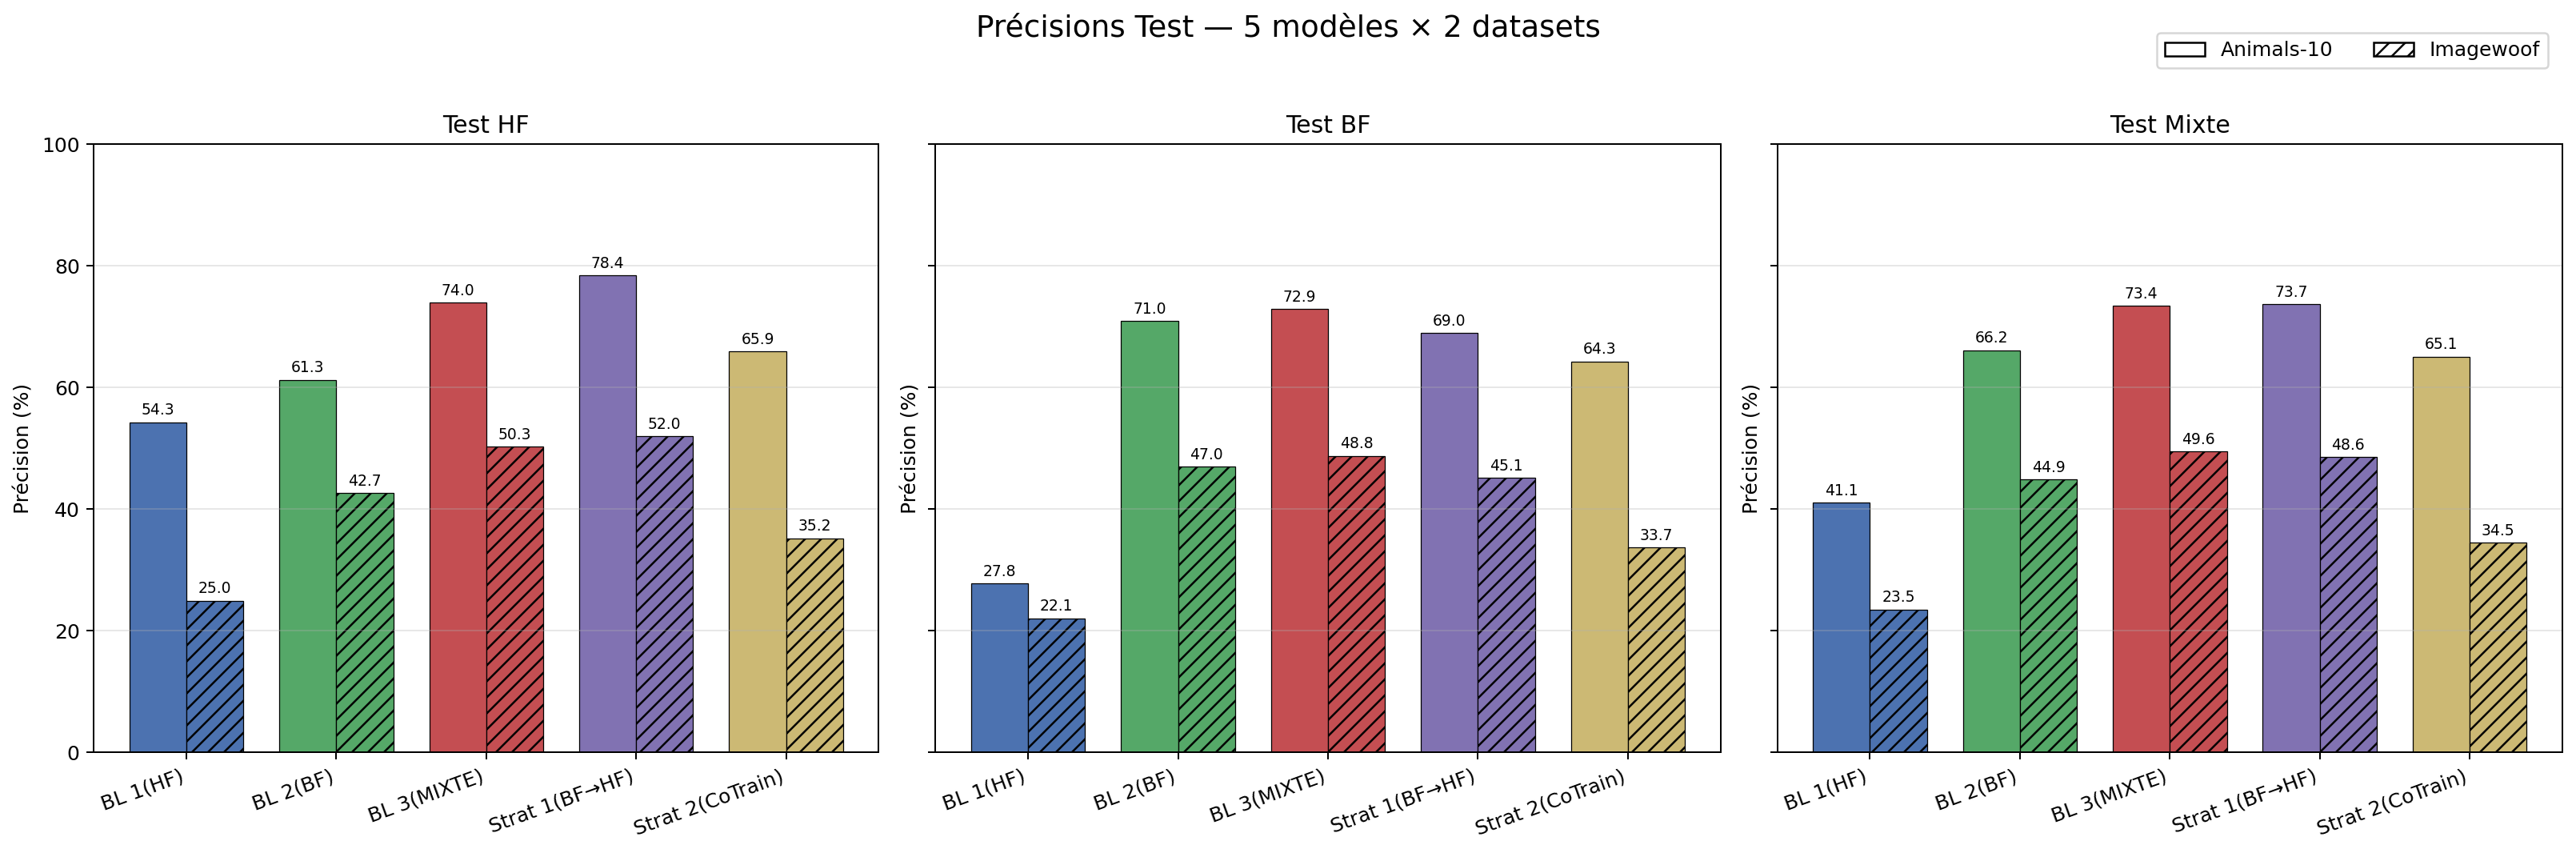
\includegraphics[width=0.98\linewidth, height=0.64\textheight, keepaspectratio]{figures/fig1_accuracy_grouped.png}
  \end{center}
  \begin{center}\footnotesize
  La hiérarchie \textbf{Strat.\,1 $>$ BL3 $>$ BL2 $>$ BL1} se conserve sur les deux datasets (valeurs plus basses sur Imagewoof, \textit{fine-grained}). Seule la Stratégie 2 décroche sur Imagewoof.
  \end{center}
\end{frame}

\begin{frame}{Classement Global \& Heatmap de Synthèse}
  \begin{columns}[T]
    \begin{column}{0.44\textwidth}
      \centering
      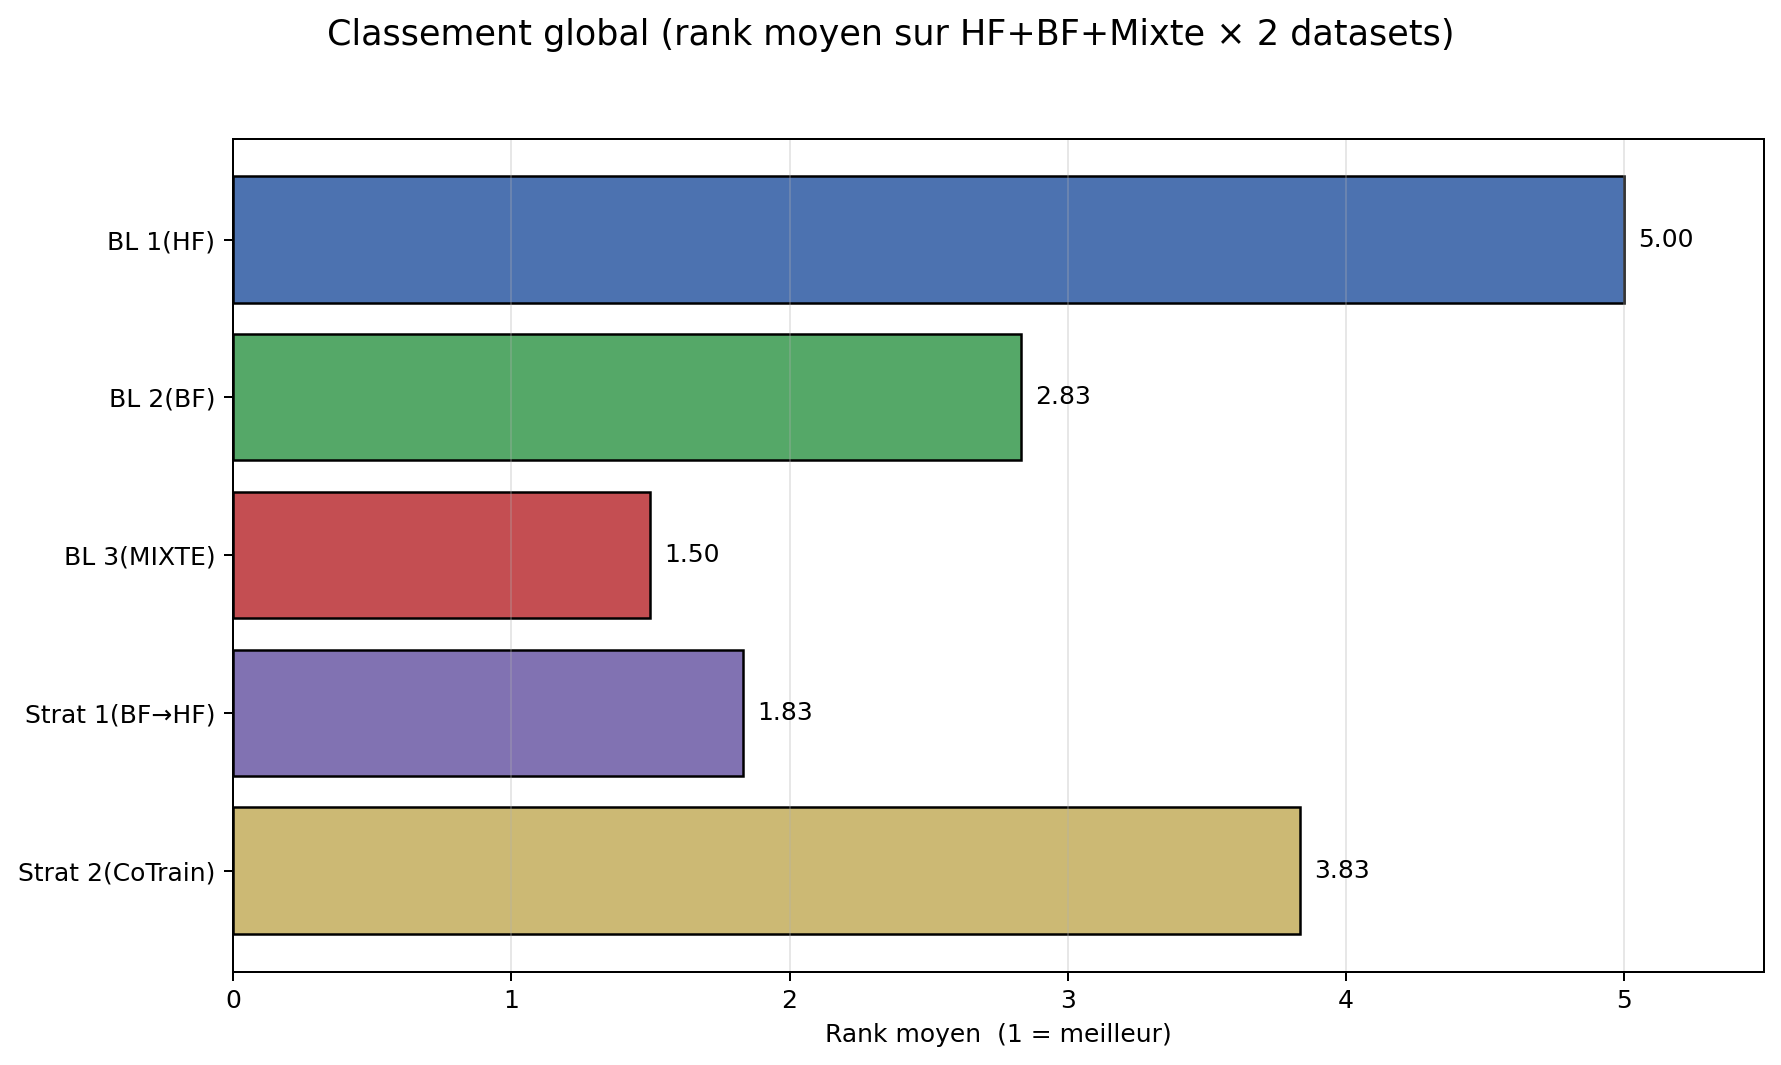
\includegraphics[width=\linewidth, height=0.62\textheight, keepaspectratio]{figures/fig8_global_ranking.png}\\[2pt]
      {\scriptsize\color{muted} Rang moyen (HF+BF+Mixte $\times$ 2 datasets)}
    \end{column}
    \begin{column}{0.55\textwidth}
      \centering
      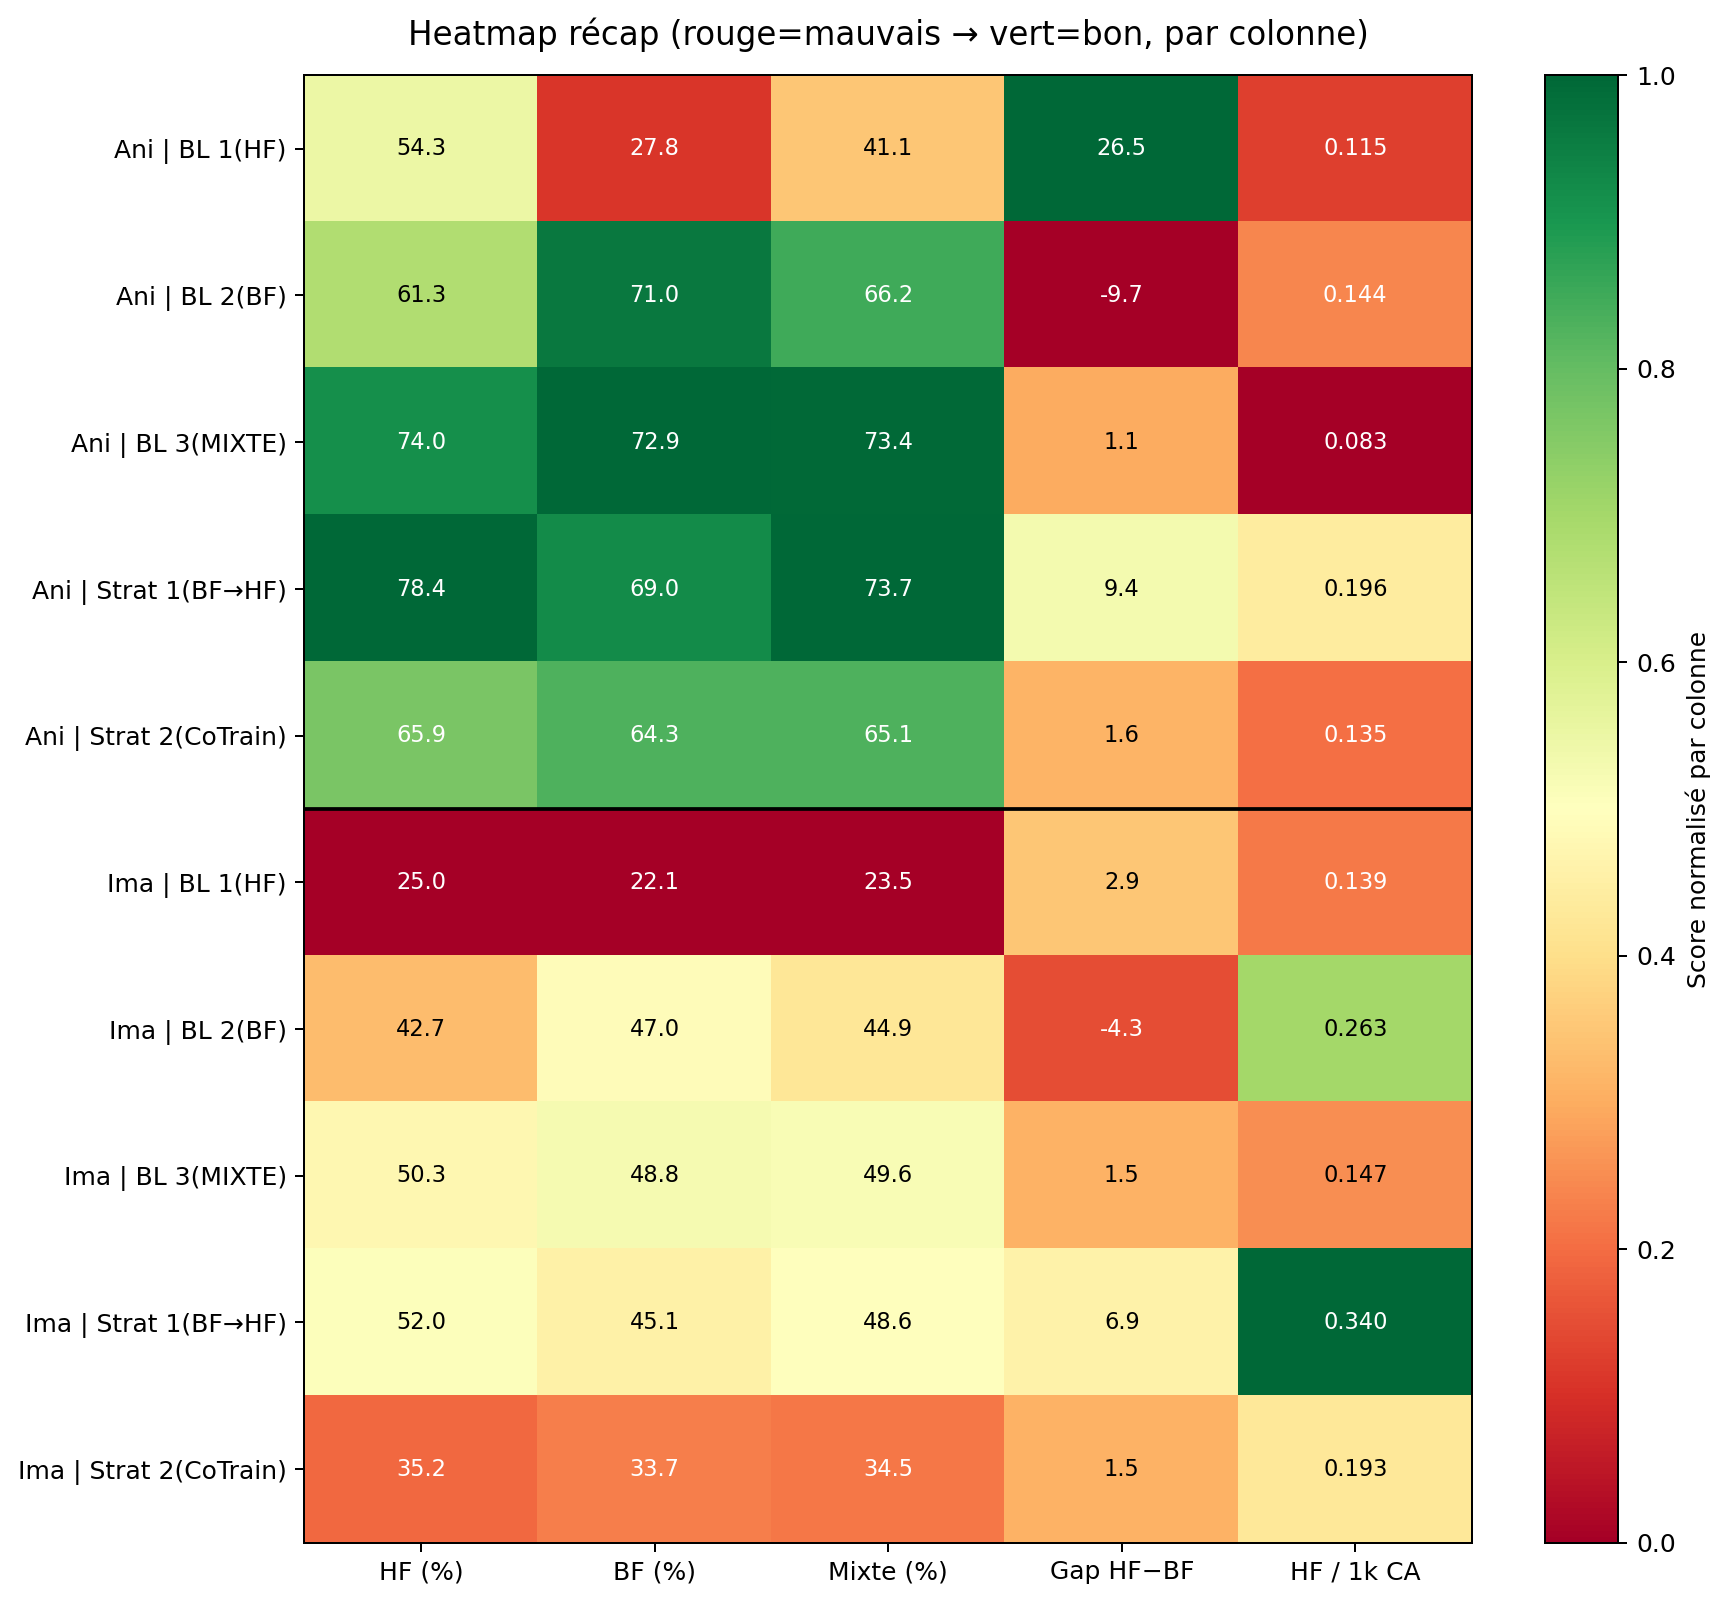
\includegraphics[width=\linewidth, height=0.66\textheight, keepaspectratio]{figures/fig5_heatmap_summary.png}
    \end{column}
  \end{columns}
  \vspace{0.1cm}
  \begin{center}\footnotesize
  \textbf{Stratégie 1} et \textbf{BL3} dominent le classement ; la heatmap synthétise toutes les métriques (vert = meilleur).
  \end{center}
\end{frame}

\begin{frame}{Compromis Coût / Précision}
\framesubtitle{Frontière de Pareto et efficacité économique}
  \begin{columns}[T]
    \begin{column}{0.50\textwidth}
      \centering
      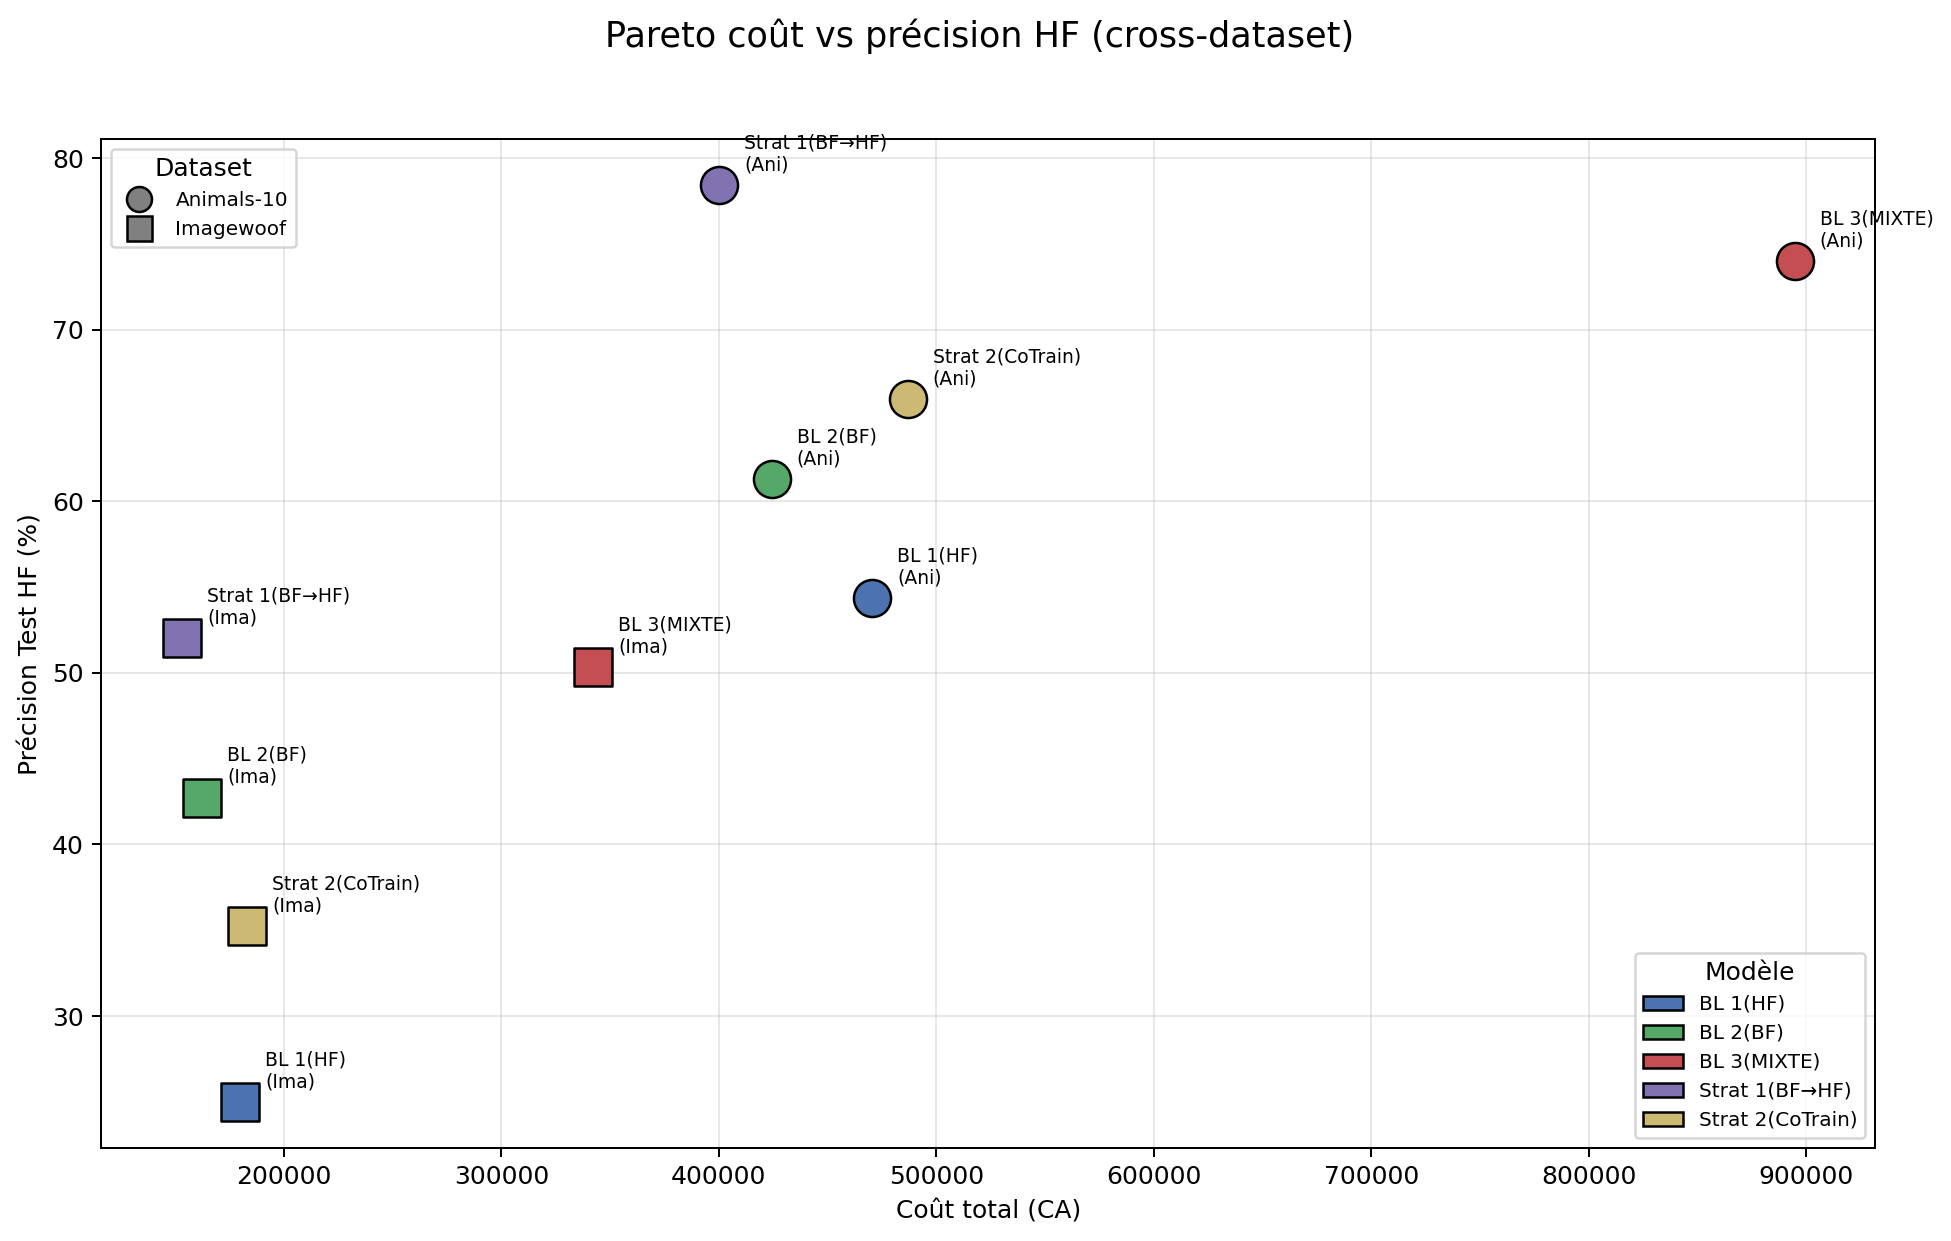
\includegraphics[width=\linewidth, height=0.60\textheight, keepaspectratio]{figures/fig2_pareto_cost_vs_accuracy.png}\\[2pt]
      {\scriptsize\color{muted} Haut-gauche = mieux (haute précision, faible coût)}
    \end{column}
    \begin{column}{0.48\textwidth}
      \centering
      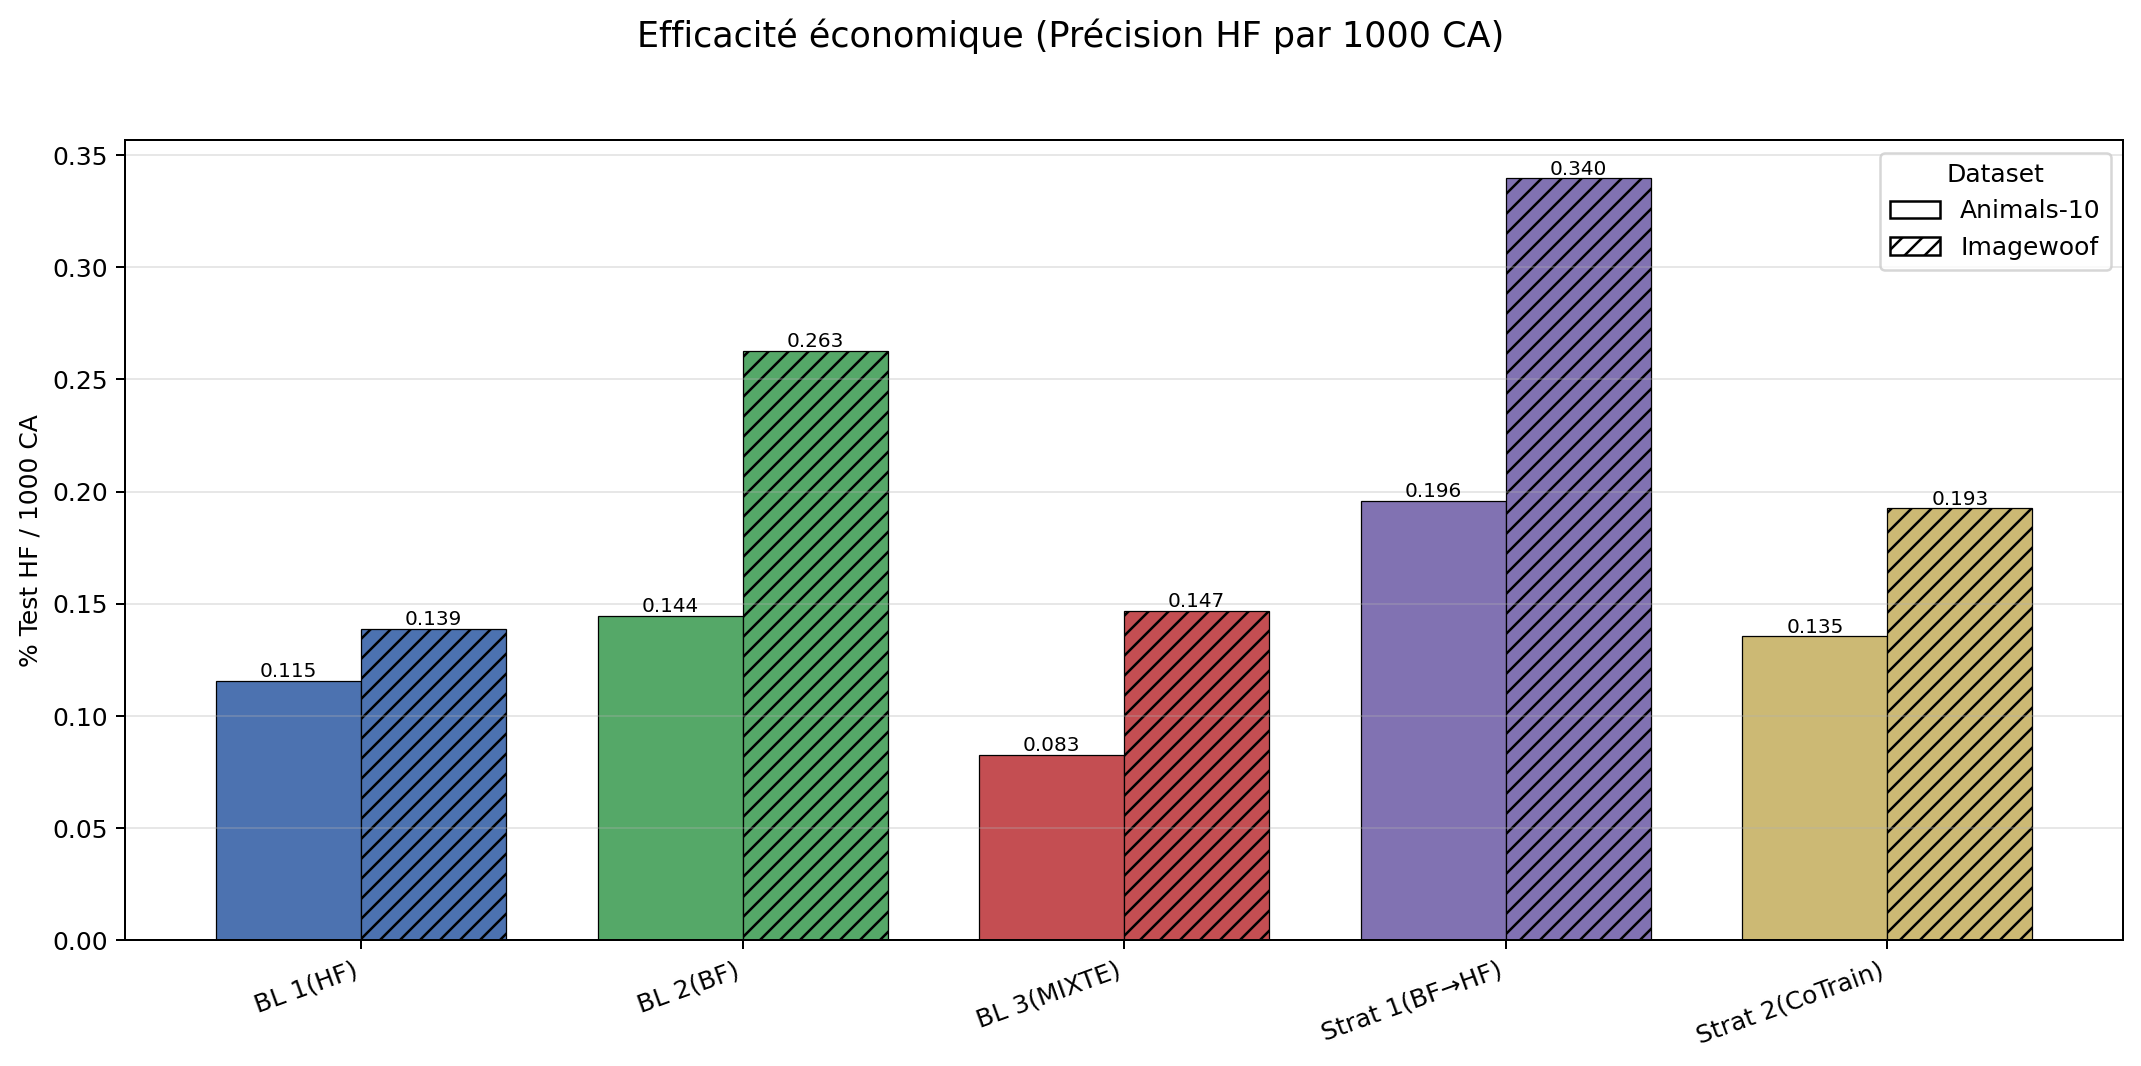
\includegraphics[width=\linewidth, height=0.60\textheight, keepaspectratio]{figures/fig4_efficiency.png}\\[2pt]
      {\scriptsize\color{muted} Précision HF par 1000 CA}
    \end{column}
  \end{columns}
  \vspace{0.1cm}
  \begin{center}\footnotesize
  À \textbf{coût données identique}, la Stratégie 1 domine BL3 : meilleure précision HF pour un \textbf{coût total / calcul $\approx$ divisé par 2}.
  \end{center}
\end{frame}

\begin{frame}{Robustesse à l'Intensité de Dégradation}
  \begin{columns}[T]
    \begin{column}{0.49\textwidth}
      \centering \textbf{\scriptsize ANIMALS-10}\\[1pt]
      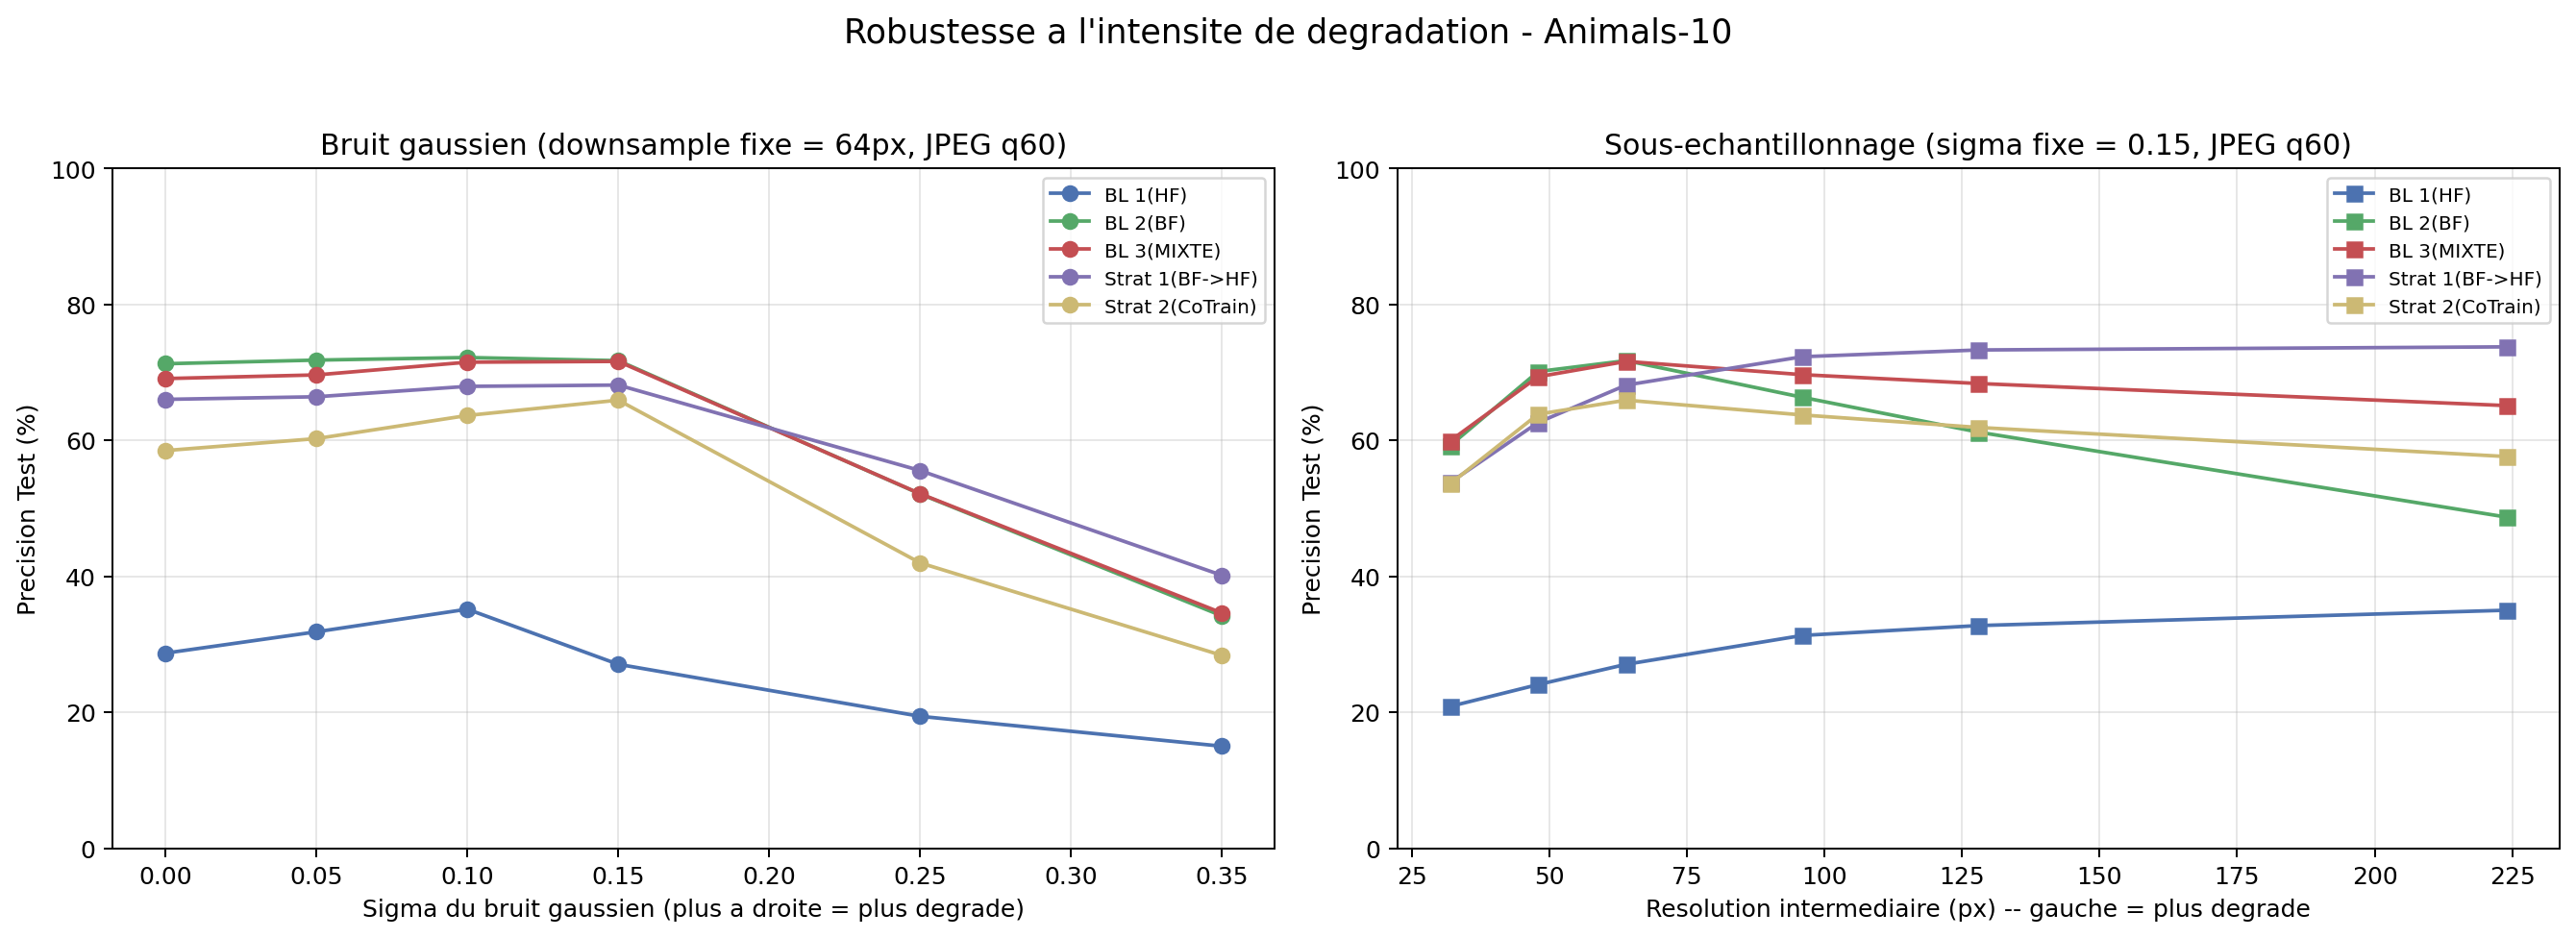
\includegraphics[width=\linewidth, height=0.52\textheight, keepaspectratio]{figures/robustness_degradation_animals.png}
    \end{column}
    \begin{column}{0.49\textwidth}
      \centering \textbf{\scriptsize IMAGEWOOF}\\[1pt]
      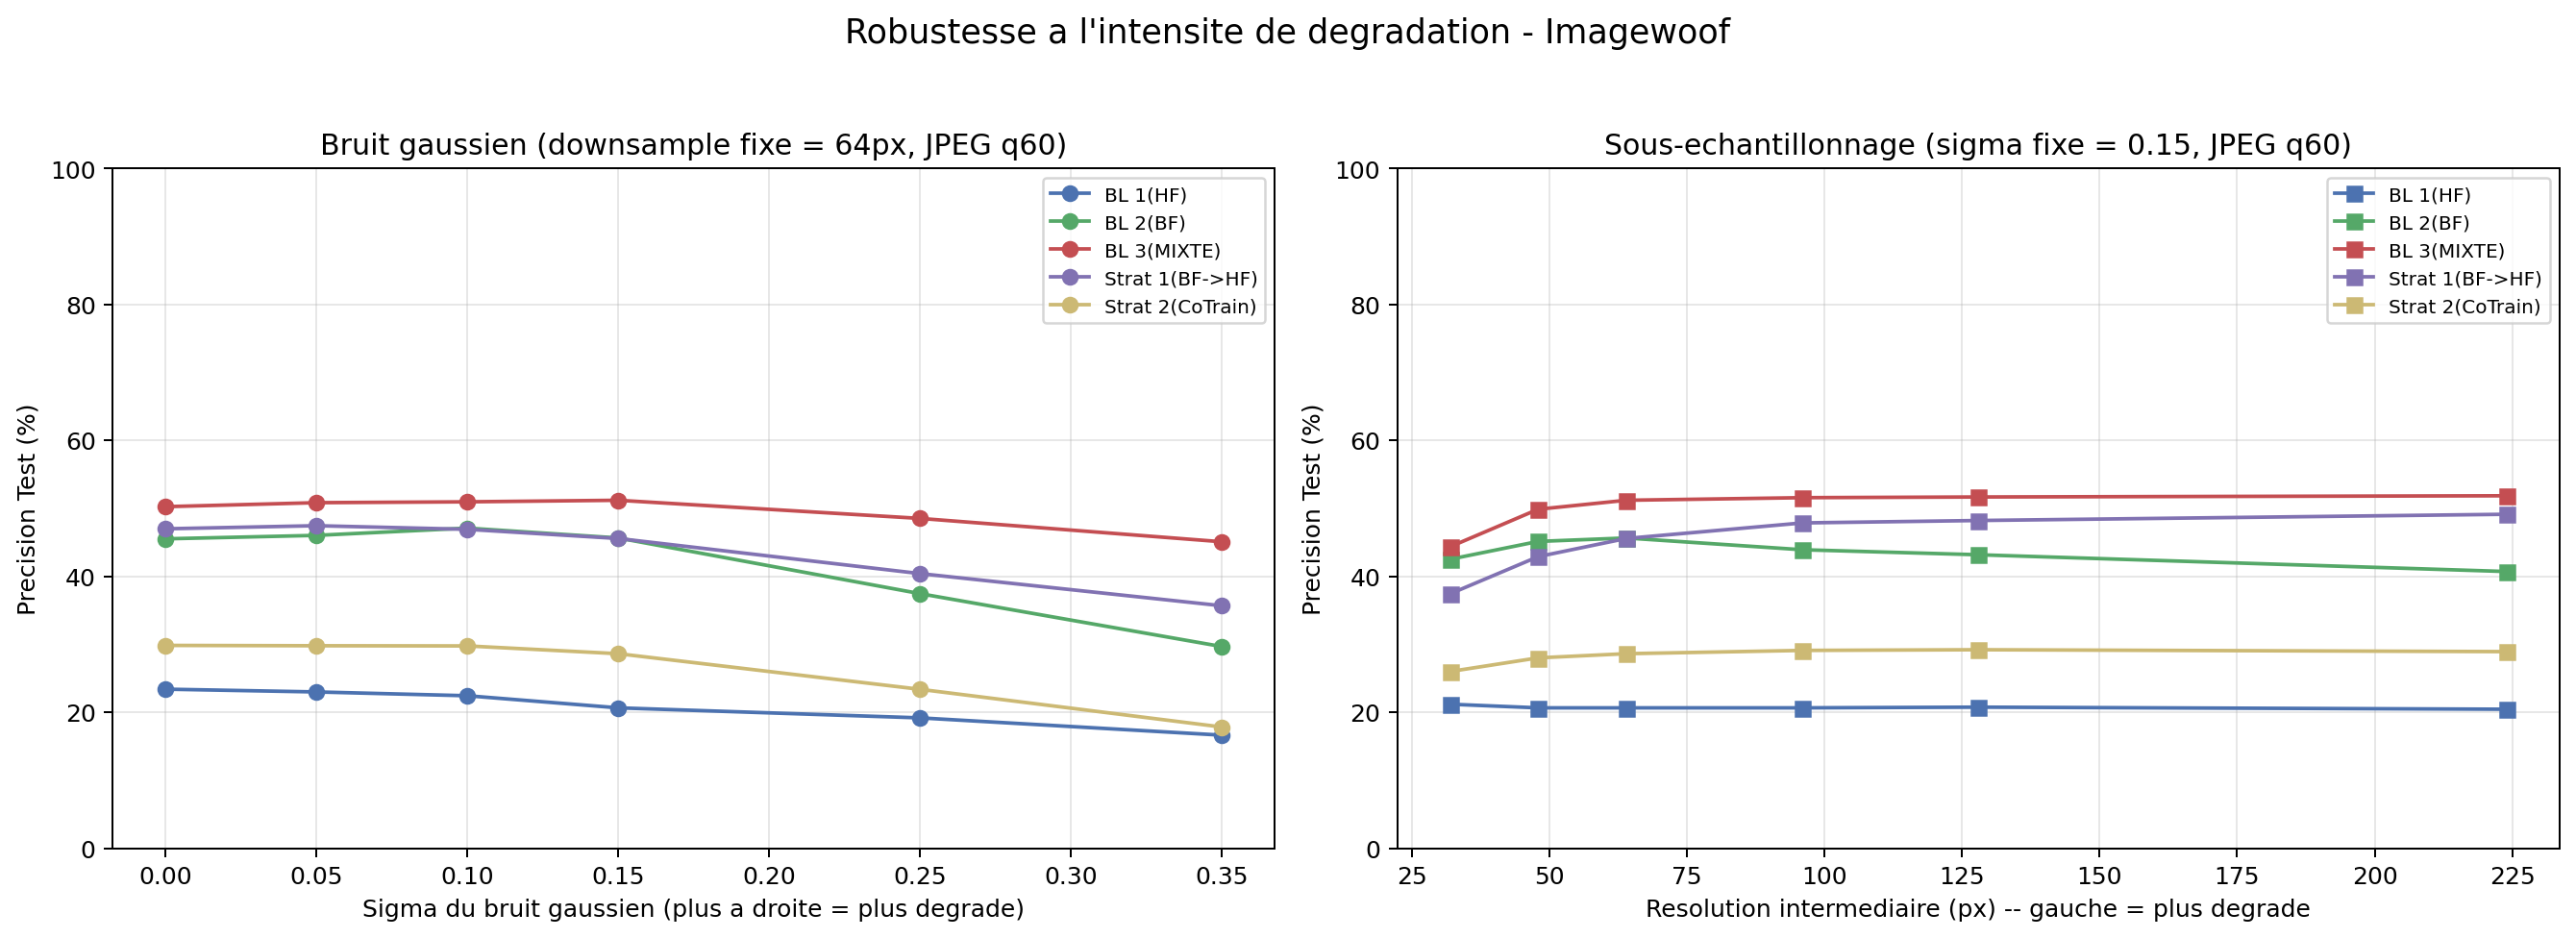
\includegraphics[width=\linewidth, height=0.52\textheight, keepaspectratio]{figures/robustness_degradation_imagewoof.png}
    \end{column}
  \end{columns}
  \vspace{0.05cm}
  \begin{alertblock}{\footnotesize Lecture}
    \footnotesize \textbf{BL1 (HF seul) est la plus fragile} : sa précision s'effondre dès l'ajout de bruit/flou. Les modèles ayant vu du BF (BL2, BL3, Stratégie 1) restent robustes jusqu'à des dégradations modérées et ne chutent qu'aux intensités extrêmes.
  \end{alertblock}
\end{frame}

\begin{frame}{Sensibilité au Ratio de Coût HF:BF}
\framesubtitle{Et si la donnée HF coûtait 5$\times$, 20$\times$, 50$\times$ le BF ?}
  \begin{columns}[T]
    \begin{column}{0.49\textwidth}
      \centering \textbf{\scriptsize ANIMALS-10}\\[1pt]
      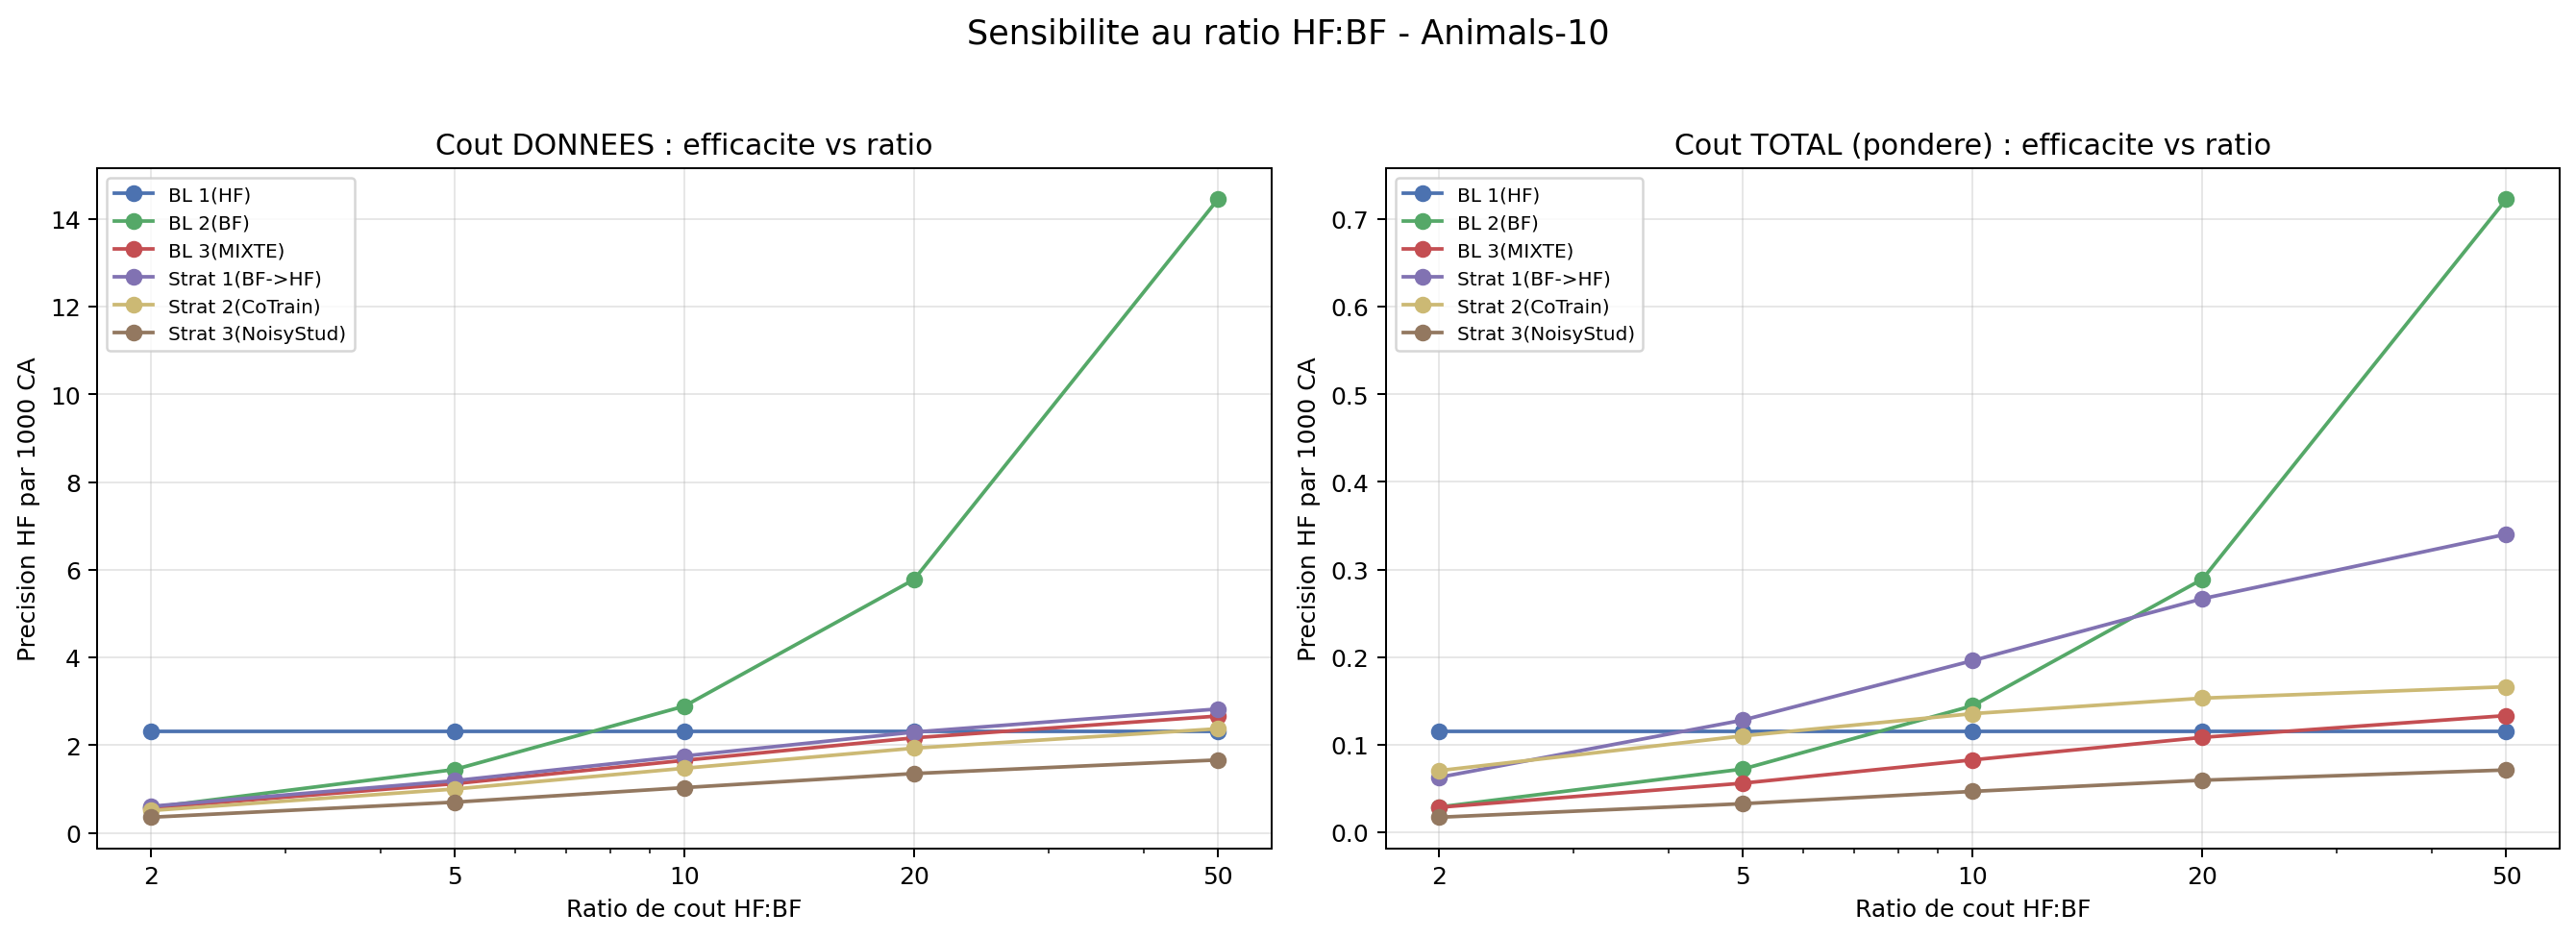
\includegraphics[width=\linewidth, height=0.52\textheight, keepaspectratio]{figures/cost_ratio_sensitivity_animals.png}
    \end{column}
    \begin{column}{0.49\textwidth}
      \centering \textbf{\scriptsize IMAGEWOOF}\\[1pt]
      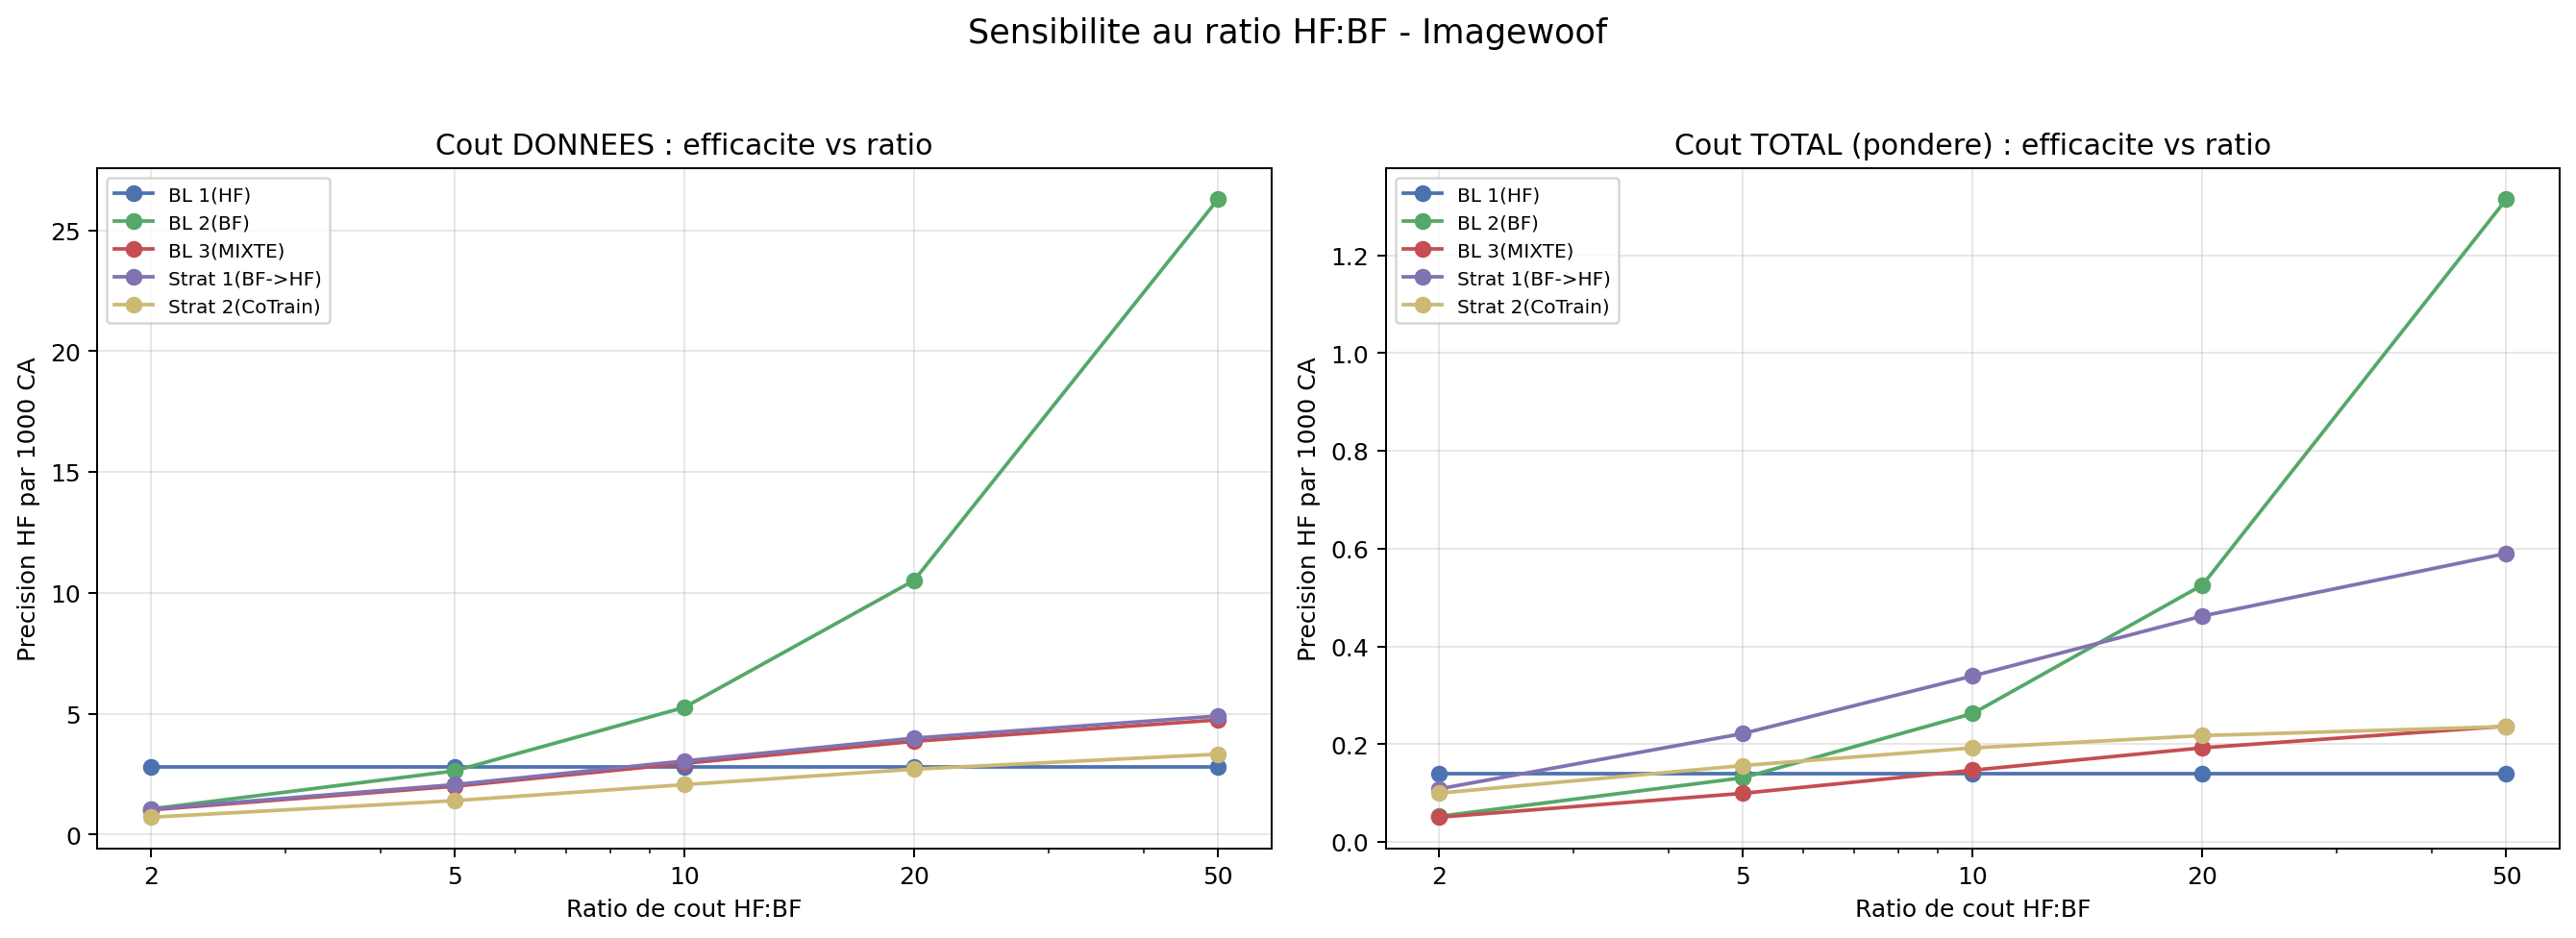
\includegraphics[width=\linewidth, height=0.52\textheight, keepaspectratio]{figures/cost_ratio_sensitivity_imagewoof.png}
    \end{column}
  \end{columns}
  \vspace{0.05cm}
  \begin{block}{\footnotesize Nuance honnête}
    \footnotesize Le modèle le plus \textbf{efficace} (précision par CA) \textit{dépend du ratio} : HF bon marché $\rightarrow$ modèles riches en HF ; HF très chère $\rightarrow$ modèles riches en BF. Mais sur la \textbf{précision HF absolue}, la Stratégie 1 reste la meilleure quel que soit le ratio.
  \end{block}
\end{frame}

% ============================================================
%  SECTION 8 : CONCLUSION
% ============================================================
\begin{frame}{Bilan et État du Rapport}

  \begin{columns}[T]
    \begin{column}{0.55\textwidth}
      \begin{block}{\footnotesize Rédaction du rapport en parallèle}
        \footnotesize \textbf{Rapport LaTeX} bientôt fini 
      \end{block}

      \vspace{0.3cm}
      \textbf{\color{primary}Prochaines et Dernières Étapes}
      \begin{itemize}\footnotesize\setlength\itemsep{2pt}
        \item Réglages fins finaux (Hyperparameter Optimization) de la Stratégie 1 (puisqu'elle est victorieuse).
        \item Finalisation du document LaTeX scientifique.
        \item Présentation Finale 
        \item Ajout d'une 3 eme méthodes ? (noisy student n'as pas fonctionné).
        \item Utilisation d'optuna 
        \item Ajout d'un 3 ème dataset ? et 4 ème ? 
        \item Ajouter matrice de confusion, identifier les classes qui souffrent le plus de la dégradation. 
        \item Conclusion et cas d'usage de ces stratégies dans le rapport. 
      \end{itemize}
    \end{column}
    
    \begin{column}{0.40\textwidth}
      \vspace{-0.2cm}
      \centering
      \begin{tikzpicture}
        \node[rounded corners=4pt, fill=success, text=white,
              minimum width=3.5cm, minimum height=1.3cm, align=center,
              drop shadow={shadow xshift=0pt, shadow yshift=-1pt, opacity=0.2}]
          {\Large\bfseries Strate 1 Vainqueur\\[1pt]\footnotesize Validée sur Fine-grained};
      \end{tikzpicture}
      
      \vspace{0.3cm}
      \begin{tikzpicture}
        \node[rounded corners=4pt, fill=accent, text=white,
              minimum width=3.5cm, minimum height=1.3cm, align=center,
              drop shadow={shadow xshift=0pt, shadow yshift=-1pt, opacity=0.2}]
          {\Large\bfseries Multi-Seeds\\[1pt]\footnotesize Confiance statistique};
      \end{tikzpicture}

      \vspace{0.3cm}
      \begin{tikzpicture}
        \node[rounded corners=4pt, fill=card, text=primary, draw=rule, line width=1pt,
              minimum width=3.5cm, minimum height=1.3cm, align=center,
              drop shadow={shadow xshift=0pt, shadow yshift=-1pt, opacity=0.2}]
          {\Large\bfseries Analyses OK\\[1pt]\footnotesize Robustesse, Pareto, Coûts};
      \end{tikzpicture}
    \end{column}
  \end{columns}

\end{frame}

\end{document}
